%%%%%%%%%%%%%%%%%%%%%%%%%%%%%%%%%%%%%%%%%%%%%%%%%%%%%%%
% Please note that whilst this template provides a
% preview of the typeset manuscript for submission, it
% will not necessarily be the final publication layout.
%
% letterpaper/a4paper: US/UK paper size toggle
% num-refs/alpha-refs: numeric/author-year citation and bibliography toggle

%\documentclass[letterpaper]{oup-contemporary}
\documentclass[a4paper,num-refs]{oup-contemporary}

%%% Journal toggle; only specific options recognised.
%%% (Only "gigascience" and "general" are implemented now. Support for other journals is planned.)
\journal{gigascience}

\usepackage{graphicx}
\usepackage{siunitx}
\usepackage{listings}

%%% Flushend: You can add this package to automatically balance the final page, but if things go awry (e.g. section contents appearing out-of-order or entire blocks or paragraphs are coloured), remove it!
% \usepackage{flushend}

\title{Training Infrastructure as a Service}

%%% Use the \authfn to add symbols for additional footnotes, if any. 1 is reserved for correspondence emails; then continuing with 2 etc for contributions.
\author[1,1a\authfn{1}]{Helena~Rasche}
\author[2]{Cameron~Hyde}
\author[3]{John~Davis}
\author[4]{Simon~Gladman}
\author[5]{Nate~Coraor}
\author[6]{Anthony~Bretaudeau}
\author[7]{Gianmauro~Cuccuru}
\author[8]{Jennifer~Hillman-Jackson)}
\author[9]{Bj\"orn~Gr\"uning}

\affil[1]{Clinical Bioinformatics Group, Department of Pathology, Erasmus Medical Center, Wytemaweg 80, 3015 CN, Rotterdam, The Netherlands}
\affil[1a]{Academie voor de Technologie van Gezondheid en Milieu, Avans Hogeschool, Lovensdijkstraat 63, 4818 AJ Breda, the Netherlands}
\affil[9]{Bioinformatics Group, Department of Computer Science, University of Freiburg, 79110 Freiburg im Breisgau, Germany}

%%% Author Notes
\authnote{\authfn{1}e.rasche@erasmusmc.nl}
\authnote{\authfn{2}Contributed equally.}

%%% Paper category
\papercat{Technical Note}

%%% "Short" author for running page header
\runningauthor{Rasche and Gr\"uning}

%%% Should only be set by an editor
\jvolume{00}
\jnumber{0}
\jyear{2020}

\begin{document}

\begin{frontmatter}
\maketitle
\begin{abstract}
%The Abstract (250 words maximum) should be structured to include the following details: \textbf{Background}, the context and purpose of the study; \textbf{Results}, the main findings; \textbf{Conclusions}, brief summary and potential implications. Please minimize the use of abbreviations and do not cite references in the abstract.
\textbf{Background:} Hands-on training, whether it is in Bioinformatics or other scientific domains, requires significant resources and knowledge to setup and run.
Trainers must have access to infrastructure that can support the sudden spike in usage, when students simultaneously run resource intensive jobs. For efficient classes, the jobs must run quickly, without queuing delays, lest they disrupt the timetable set out for the class. Often times this is achieved via running on a private server where there is no contention for the queue, and therefore no or minimal waiting time. However, this places a significant pre-requisite knowledge barrier for teachers, who must spend time learning deployment and management of compute resources. This presents significant burdens to potential training events, in terms of infrastructure cost, person-hours of preparation, technical knowledge, and available staff to manage such events. Lastly, with the advent of hybrid teaching, with groups following a broadcast instructor, it is impossible to know efficiently how students are doing, without constant teaching interruptions to inqiure if students are progressing without issue.

\textbf{Findings:} Originally developed by the Gallantries and Galaxy Europe, together with Galaxy Austrlia, and Galaxy Main we have jointly developed and iterated upon the concept of Training Infrastructure as a Service (TIaaS), a method by which to provide Training Infrastructure in a dynamic way, providing easy accessible training resources for courses and events. Event organisers request resources for a training and Galaxy administrators can allocate private queues specifically for that event. Trainees are transparently placed in a private queue where their jobs run without delay. Trainers access the dashboard of the TIaaS Service and can remotely follow the progress of their trainees without in-person interactions.

\textbf{Conclusions:} TIaaS provides reusable and fast infrastructure for Galaxy training. The instructor dashboard provides visibility into class progress, making in-person trainings more efficient and remote training possible and easy. This has provided an excellent environment for learning, as students can continue using the same server after a course ends, retaining access to their tutorials, providing good continuity for students adapting from training environments into production systems. While initially developed for hybrid courses where there was no visibility into student progress, it has also been extremely effective during completely remote courses providing unparalleled visibility for teachers. In the past 24 months, $>360$ trainings with over 18,000 trainees have used this infrastructure for training. TIaaS itself is an extension to Galaxy which can be deployed by any Galaxy administrator to provide similar benefits for their users. \url{https://github.com/galaxyproject/tiaas2}
\end{abstract}

\begin{keywords}
Galaxy; Training; Teaching; Remote Training
\end{keywords}
\end{frontmatter}

\section{Findings}
\subsection{Background}

% The background section should be written in a way that is accessible to researchers without specialist knowledge in that area and must clearly state---and, if helpful, illustrate---the background to the research and its aims. The section should end with a brief statement of what is being reported in the article.

With the volume of bioinformatics data becoming available, the availability of training for bioinformaticians is not keeping up (\cite{Attwood2017}).
The Galaxy platform \cite{afgan2018galaxy} provides one such infrastructure on which to conduct trainings, as it provides a user-friendly web-based interface to command line tools. With a wide range of tools across bioinformatics domains and beyond, and pre-existing popularity within the life sciences community, it is an ideal platform for training (\cite{gtn}).

The Galaxy community has developed a wide array of hands-on training materials (275+) covering bioinformatics and beyond (\cite{training-site}) in an attempt to combat this issue, but in order to run these tutorials at scale, one occasionally needs access to significant resources. The quite popular ``Reference-based RNA-Seq data analysis'' tutorial uses the STAR aligner (\cite{Dobin2012}), and while an ultra-fast aligner is ideal during training, it also consumes $\approx$32 GB of RAM at minimum\footnote{Many tools have similar requirements; on UseGalaxy.eu, 83 tools require $>$64 GB RAM, 151 require more than $>$32 GB, a limiting factor especially for smaller training infrastructures. Even with a large cluster, many trainees can still consume all of the available overhead.}. While individual STAR jobs might execute successfully, the infrastructure remains a limiting factor for scaling up to medium or large training events, presenting unexpected delays due resource contention. When jobs must queue, this significantly impacts a training's timeline to the deteriment of students. While the teacher could alternatively deploy their own private infrastructure, this requires significant additional knowledge, time, and energy. Both alternatives result in significant barriers for potential, motivated trainers who wish to give a Galaxy or bioinformatics training course.

During one of the initial Gallantries events, which was the first forray for UseGalaxy.eu trainers into hybrid training--wherein we had three classrooms spread across the Netherlands, Germany, and Greece--we discovered significant pain points teaching remote courses and getting efficient feedback. Normally teachers of this style of hands-on lesson wander around the classroom to check that students are progressing acceptably, or use the Carpentries method of red and green post-it notes to let students communicate if things are going well or poorly. This was difficult in this situation as on-site staff needed to survey they room and report back centrally to the teacher, however it was completely impossible in fully remote training events such as have been occurring for the last 3 years of the pandemic.

\subsection{Results}

We initially developed Training Infrastructure as a Service (TIaaS) initially to solve our primary problems of ensuring we could quickly setup training resoures which would be private to a single course. By re-using an existing public server backed by significant compute resources, we completely remove the infrastructure setup and maintenance costs of hosting an event for trainers. While individual TIaaS deployments can handle job scheduling differently, they all allocate private resources so jobs can always run without delay. Lastly, provides good separation of responsibilities between trainers who are teaching and the server administrators responsible for Galaxy, rather than requiring teachers to be cross-trained in administration. The live dashboard showing student jobs provides unparalleled visibility into student progress and any potential issues a teacher should discuss with students. We have shared this service with the Galaxy training community to overwhelmingly positive feedback.

\begin{figure}[bt!]
\centering
\includegraphics[width=\linewidth]{images/dashboard.png}
\includegraphics[width=\linewidth]{images/queue.png}
\caption{The top of the training dashboard page shows the status of the jobs in the past hours. A heatmap of the tools which were run indiciates if everything is running smoothly or if there is anything the trainer should look into. As trainees follow along and run different tools these show up immediately, allowing trainers to identify if everyone has started or finished a specific step.. The bottom image shows the rest of the training dashboard, which lists jobs that were run chronologically, colour coded first by user, and second by the job status. Randomized colours are used to protect user privacy, as we wanted dashboards to be visible to course members.}\label{figure:dashboard}
\end{figure}

We implemented a web service, and separately job scheduling rules, which function together to present a private queue for users in specific Galaxy user groups. Trainers register their course and teaching materials with an online form. Administrators review training requests, using information about their class size, the tools used in those training materials, and the resource allocations of those tools on the infrastructure to estimate the required compute resources.

If space is available and any other site specific criteria is met, the training can then be approved. Next, administrators (optionally) deploy additional private compute resources, or allocate existing resources, in a local compute environment and attach them to their existing Galaxy scheduling, via the job scheduling rules. Administrators can then provide trainers with a URL such as \url{https://usegalaxy.eu/join-training/test}, and the trainer can then in turn provide to their trainees. When training participants access the URL, they are registered in the TIaaS system, without the service administrator or trainers needing to be aware of users identities to aid in privacy protection\footnote{Local deployments can choose to disable that, e.g. for Galaxies deployed within a university or highschool where attendee privacy is not a requirement.}. The job scheduler, once aware of the training group, will place any job run by someone in that training onto the private training nodes (Figure \ref{figure:queue}).

\begin{figure}[bt!]
\centering
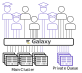
\includegraphics[width=\linewidth]{images/rules.png}
\caption{All jobs are processed by the same Galaxy server, but jobs from users in the training groups receive special handling. These jobs are allowed to run on the protected training resources (purple). If the training resource is full, these jobs can spill over to the main queue if necessary.}\label{figure:queue}
\end{figure}

The course dashboard, visualising the progress of participants (Figure \ref{figure:dashboard}), has significantly improved the lives of trainers, especially situations involving remote participants. The dashboard provides instantaneous, aggregated, and pseudonymised feedback for the trainers into how their trainees are progressing. It has also enabled remote and hybrid trainings to take place, which were previously very labour intensive due to necessity of maintaing insight into potential issues across multiple locations. Requiring students to regularly provide up-to-date information on how participants are progressing does not work effectively in practice with low student response rates. With the training dashboard, howver, this is unnecessary as course staff can watch student progress in real time. Teachers can see if steps are completed successfully on average, or if there are many issues and they might need to pause or explain the step in more detail.

\subsubsection{Usage}
Since the introduction of TIaaS in July 2018, it has seen nearly constant use with more than 110 trainings occuring on the platform, all across the world (Figure \ref{figure:map}). Everything from one day workshops for bioinformaticians to multi-month courses for highschool students have been hosted by TIaaS and UseGalaxy.eu, covering topics such as HTS, RNA-Seq, ChIP-Seq, Imaging Analysis, Proteomics, and Machine Learning.

\begin{figure}[bt!]
\centering
\includegraphics[width=\linewidth]{images/map.png}
	\caption{Since its introduction, TIaaS has seen worldwide usage despite--or perhaps in some cases due to--the server being hosted in Germany. This dashboard is part of the TIaaS platform, allowing deployers to share their numbers with funding agencies and the world.}\label{figure:map}
\end{figure}

Class sizes have ranged considerably, from the median of 15 participants to a maximum of 3000 registrants at a fully asynchronous course. Most courses were short training events with a median of two days, however some ran for multiple months like a number of highschool courses which used TIaaS over the entire semester. The variability in administrator deployments of TIaaS can allow it to accommodate a wide range of teaching scenarios; for some courses large resources may be allocated like the Galaxy Community Conferences where the big three Galaxies configued TIaaS with considerable resources to permit local and remote synchronous training, all the way to semester long courses which may not necessitate a large amount of resources.

\section{Methods}

\subsection{Implementation}
TIaaS was written in Python with the Django framework. It has been designed from the start to have a very limited scope: provide a form to register events, an approval flow for administrators, and a connection to the Galaxy database to manage user-group relationships when needed.

For instructors a form is provided (\texttt{/tiaas/new}) which permits them to register a new training event. When submitted, this goes into the associated database. Administrators can view the requested training events and approve or reject them using the built in Django admin interface. When users visit their their training url (\texttt{/join-training/<id>}) the system accesses their Galaxy session cookie, and decodes it. They are automatically registered as part of a Galaxy group named after the training (e.g. \texttt{training-<id>}) which is created on demand.

When visiting the dashboard (Figure \ref{figure:dashboard}), the training ID is extracted from the URL (e.g. ``test'' from \url{https://usegalaxy.eu/join-training/test/status}), and all non-terminal jobs, in the past 1-6 hours, from those users are presented in a pseudonymised manner.

When a job is submitted by a user in a training group, the Galaxy instance's job scheduling system system reads the user's groups and roles, and if any of these include something prefixed with \texttt{training-}, then this is converted to a job scheduler specific requirement string (Figure \ref{code:scheduler}). Ideally these are constructured to prefer training nodes, and spill over to the main queue if training nodes are full, but this feature is dependant on specific scheduler capabilities.

\begin{figure}[!ht]
\centering
\begin{lstlisting}[frame=single,language=Python]  % Start your code-block
def queue_job(job, user):
    job.cluster = 'main'

    if inTrainingGroup(user):
        training = getTrainingGroup(user)
        job.cluster = training

    return job
\end{lstlisting}
\caption{Python pseudocode representing how TIaaS jobs are typically processed and allocated to a private queue.\label{code:scheduler}}
\end{figure}

\subsection{Deploying}
As the Galaxy community has largely settled on Ansible for deployment of Galaxy, and related components, an Ansible role was produced for deploying the TIaaS Service. A few known deployments make their configuration public, and we can see the differences: one the motivating factor in TIaaS' design was such flexibility. \emph{Galaxy Europe} uses it with HTCondor, and job rules that allow ``failover'' to the main cluster, new machines are brought up in an OpenStack cluster specifically for training events and destroyed aftewards. Each Machine is tagged with an HTCondor attribute indicating which training it belongs to, and the job rules\footnote{Visible in \url{https://github.com/usegalaxy-eu/infrastructure-playbook/blob/930bbafe5f743afa642015a4771086b390d53ad8/files/galaxy/dynamic_rules/usegalaxy/sorting_hat.py#L327-L337}} use that to enable access to those machines, and a preference for them. \emph{Galaxy Australia} has a separate ``training cluster'' in their OpenStack deployment, and route all training jobs to the single shared cluster\footnote{Visible at \url{https://github.com/usegalaxy-au/infrastructure/blob/63a1111e3231466cbc59378dcb6dc5ceac97d507/files/galaxy/dynamic_job_rules/dev/dynamic_rules/destination_mapper.py#L37-L44}}. \emph{Galaxy Main} takes a different approach, lacking additional clusters but having an excellent queueing system, they artificially limit the runtime, memory, and CPU resources allocated to users running jobs within a TIaaS group. \emph{Avans Hogeschool} uses TIaaS in an internal Galaxy where they provide no preferential treatment, and just use the dashboard to observe students.

\subsection{Future Work}
 This system can be generically useful for temporary and private compute resources, but is currently focused on training use case.

\section{Availability of source code and requirements}

\begin{itemize}
\item Project name: ~Training Infrastructure as a Service
\item Github repository:~\url{https://github.com/galaxyproject/tiaas2/}
\item Admin Training Manual: ~\url{https://training.galaxyproject.org/training-material/topics/admin/tutorials/tiaas/tutorial.html}
\item Teacher Training Manual: ~\url{https://training.galaxyproject.org/training-material/topics/instructors/tutorials/setup-tiaas-for-training/tutorial.html}
\item Operating system(s): ~Unix
\item Other requirements: ~Galaxy version 18.01 or higher
\item License: ~GNU AGPL-3.0
\end{itemize}

\section{Availability of supporting data and materials}
All code is open source and available on GitHub (https://github.com/galaxyproject/tiaas2).

\section{Declarations}

\subsection{List of abbreviations}
\begin{itemize}
\item TIaaS: Training Infrastructure as a Service
\end{itemize}


\subsection{Competing Interests}
The authors declare that they have no competing interests.

\subsection{Funding}
This project is funded with the support of the Erasmus+ programme of the European Union (Grant 2020-1-NL01-KA203-064717).
This project was made possible with the support of the Albert Ludwig University of Freiburg.
The work is in part funded by Collaborative Research Centre 992 Medical Epigenetics (DFG grant SFB 992/1 2012) and German Federal Ministry of Education and Research (BMBF grants 031 A538A/A538C RBC and 031L0101B/031L0101C de.NBI-epi). The article processing charge was funded by the Baden-Württemberg Ministry of Science, Research and Art and the University of Freiburg in the funding programme Open Access Publishing.

\subsection{Author's Contributions}
HR and BG conceived of the presented idea. HR carried out the implementation. Significant improvements were later made by CH, JD, and AB. HR and BG contributed to the writing of the manuscript.

\section{Acknowledgements}
The authors would like to thank the Galaxy community for their enthusiasm for this project, and their feedback on each iteration.

%% Specify your .bib file name here, without the extension
\bibliography{paper-refs}

\end{document}
